\documentclass[12pt]{exam}
%\documentclass[12pt]{article}
\usepackage[letterpaper, margin=0.75in]{geometry}
\usepackage{graphicx}
\usepackage{enumitem}
\usepackage{booktabs}
\usepackage{amsmath}
\usepackage{tabularx}
\usepackage{color}

\begin{document}
\footer{}{Page \thepage\ of \numpages}{}

\begin{flushright}
\makebox[0.5\textwidth]{\large Name:\enspace\hrulefill}
\vspace{0.2in}

\makebox[0.5\textwidth]{\large Date:\enspace\hrulefill}
\end{flushright}

\begin{center}

\includegraphics[width=10cm]{../images/logo.png}
\end{center}

\begin{center}
\noindent{\LARGE Conceptual Physics \\ Class 14 Questions \\ May 11th, 2018  \\ ~ \\  Practice Questions for Second Partial Test}
\end{center}

\vspace{0.2in}


\begin{center}
\noindent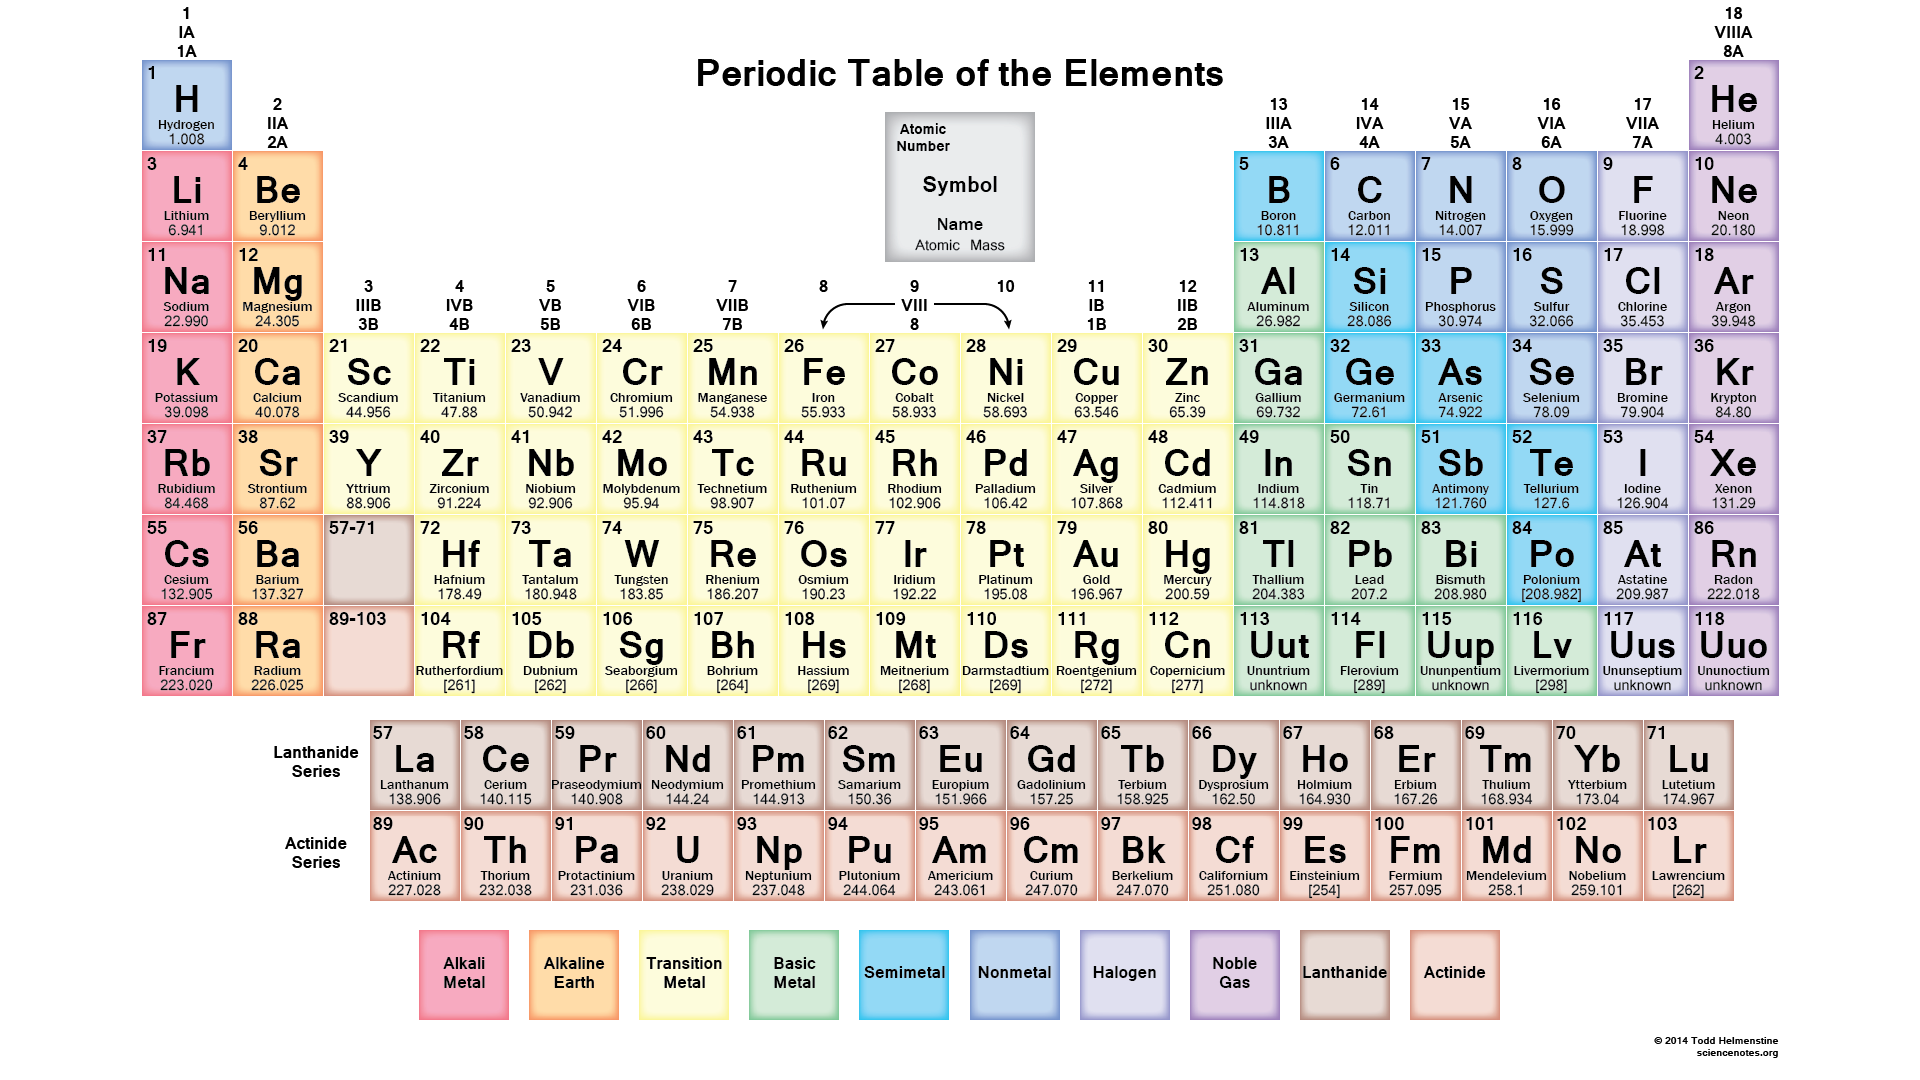
\includegraphics[width=\textwidth]{../images/periodicTable.png}
\end{center}

\begin{center}
\noindent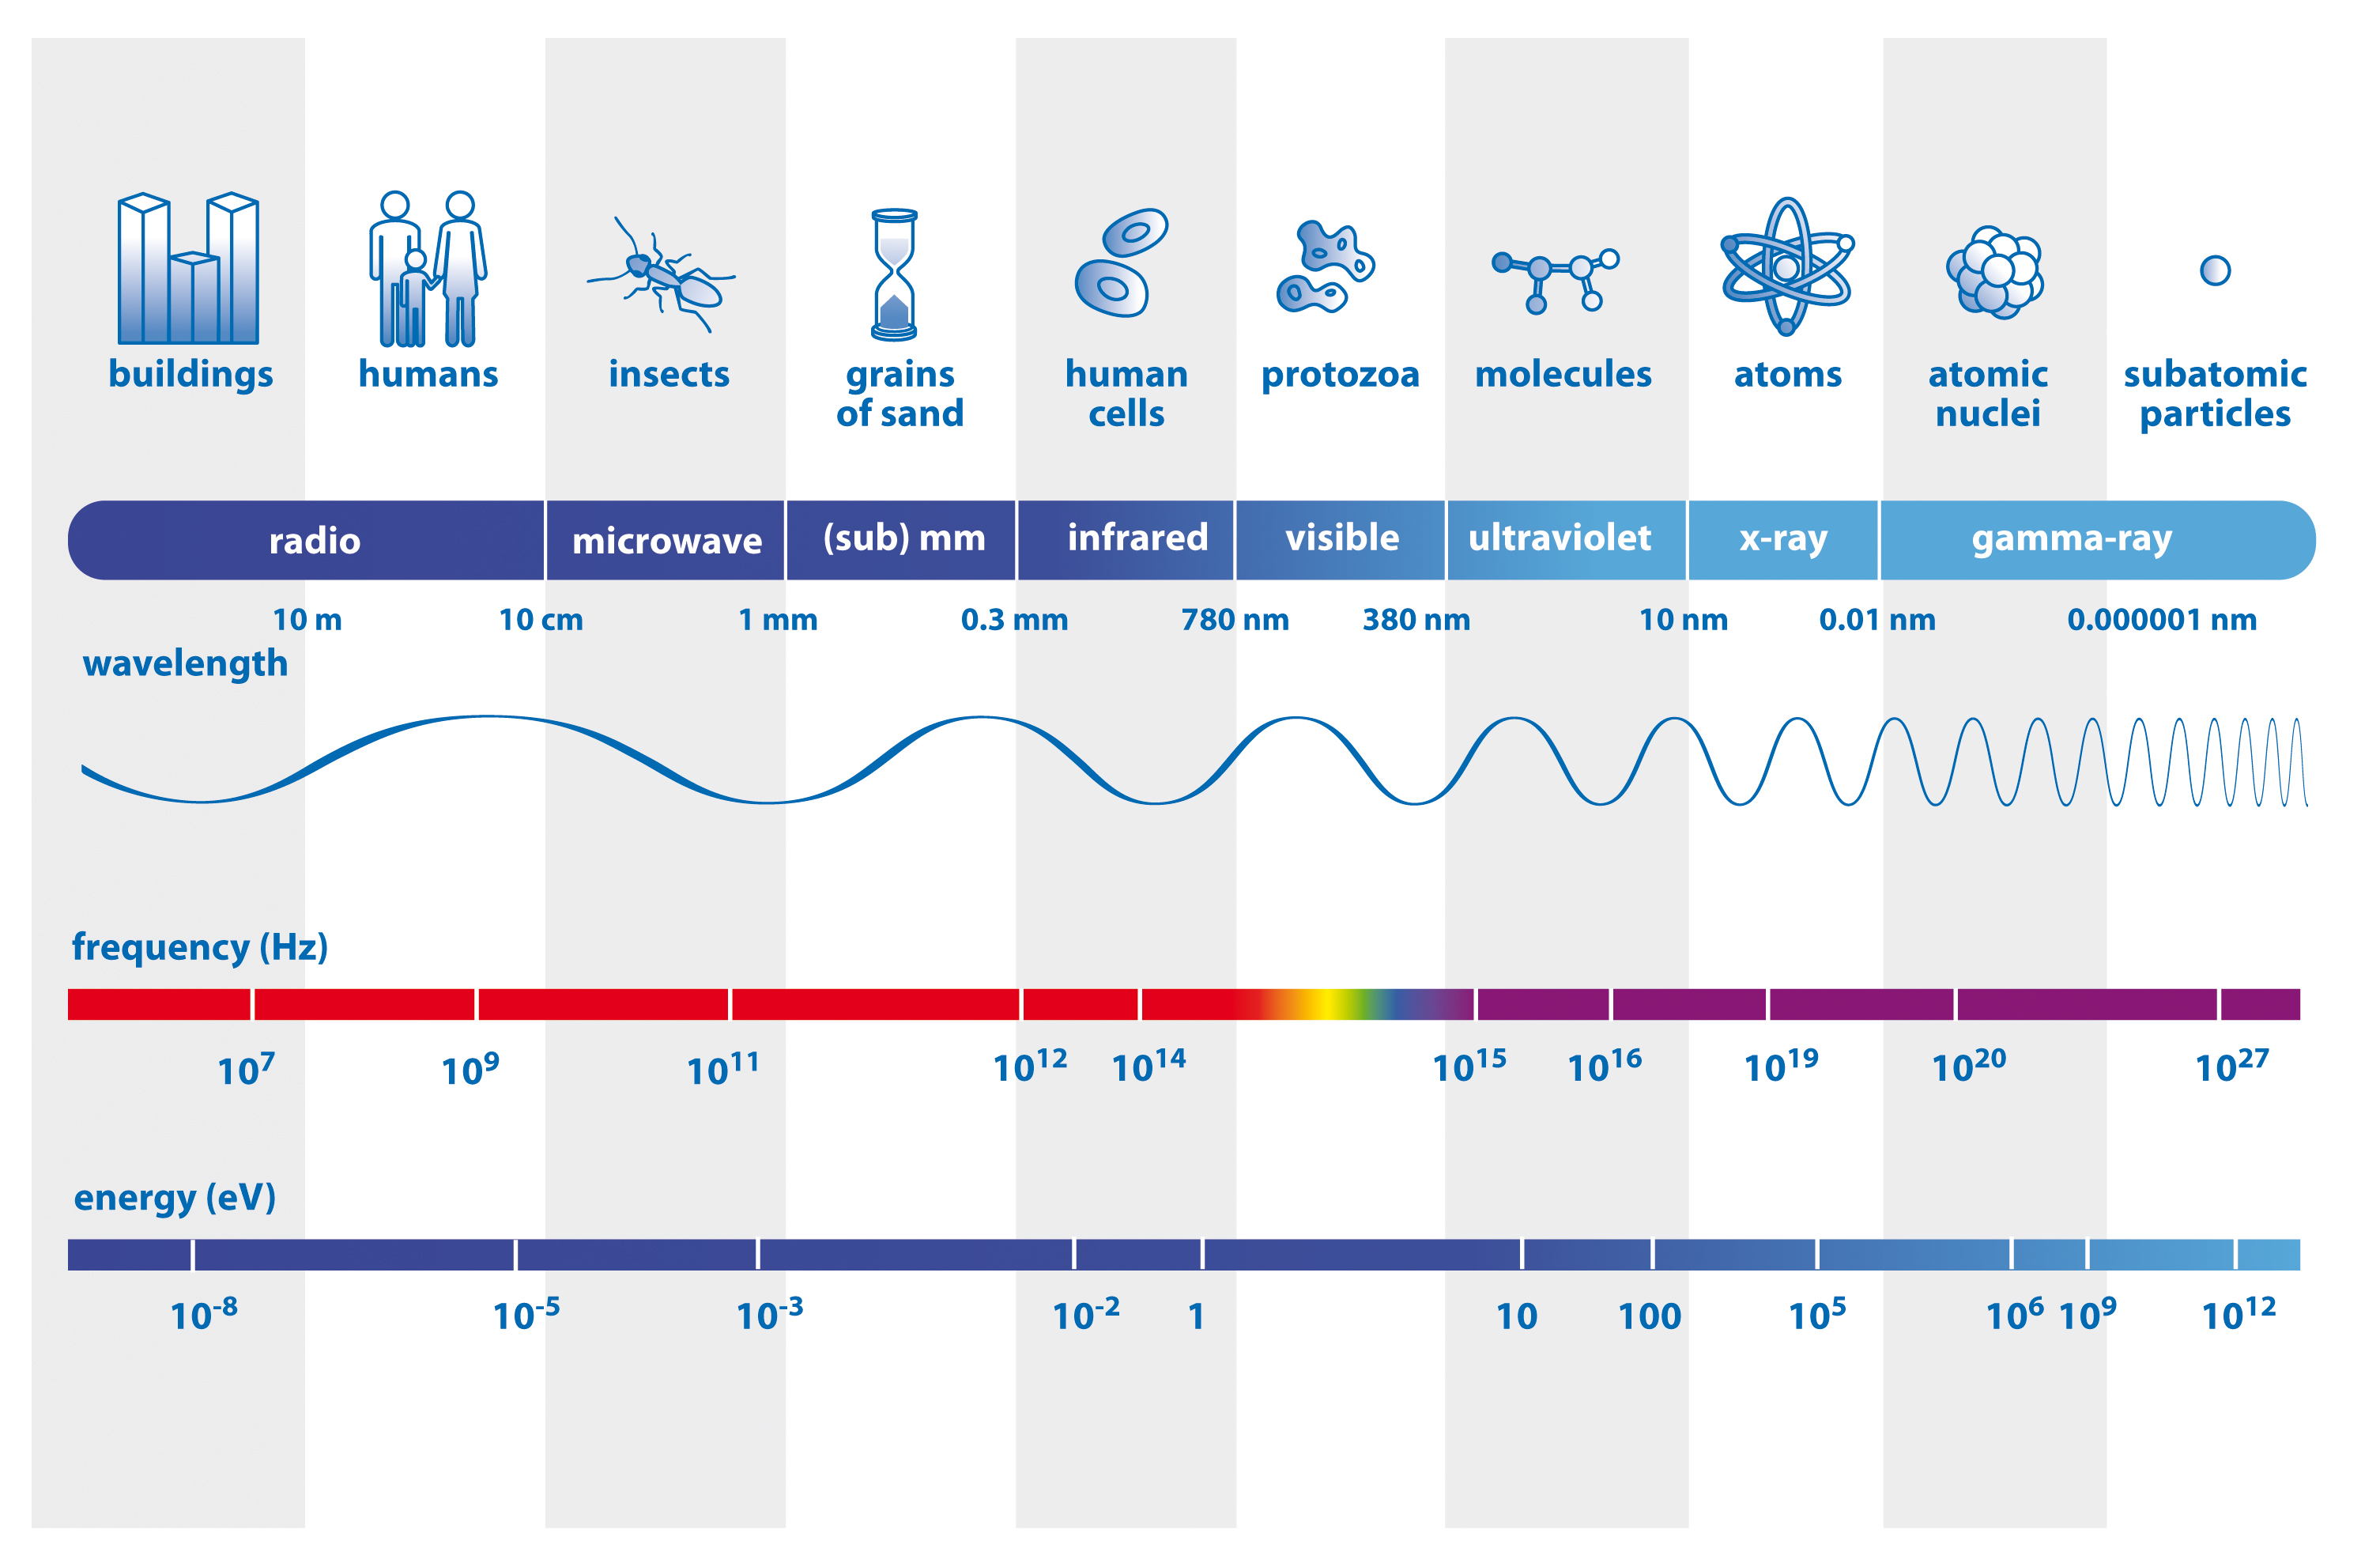
\includegraphics[width=\textwidth]{../images/emSpectrum.jpg}
\end{center}

\clearpage

\begin{questions}
\question Four point charges are arranged in 2 different configurations, resulting in different electric fields. Assume that the size of all charges are the same, and consider only the fact that some are positive and others are negative.

\begin{parts}

\part Draw the \textbf{electric} field lines around the following:
\vspace{0.25in}
\begin{center}
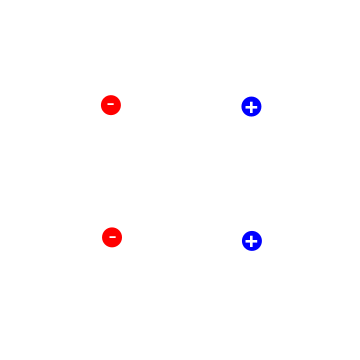
\includegraphics[width=3in]{../images/4chargesA.png}
\end{center}
\vspace{0.25in}

\part  Draw the \textbf{electric} field lines around the following:
\vspace{0.25in}
\begin{center}
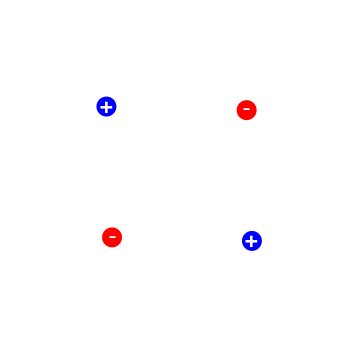
\includegraphics[width=3in]{../images/4chargesB.png}
\end{center}
\vspace{0.25in}

\clearpage
\part Draw the \textbf{gravitational} field lines around the following:
\vspace{0.25in}
\begin{center}
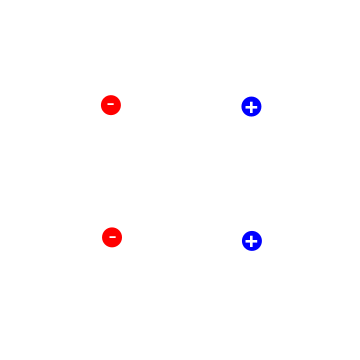
\includegraphics[width=3in]{../images/4chargesA.png}
\end{center}
\vspace{0.25in}

\part  Draw the \textbf{gravitational} field lines around the following:
\vspace{0.25in}
\begin{center}
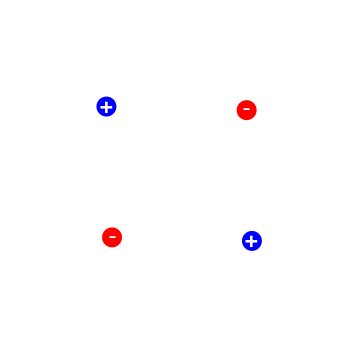
\includegraphics[width=3in]{../images/4chargesB.png}
\end{center}
\vspace{0.25in}
\end{parts}

\clearpage
\question Astronauts on three different spaceships are communicating with each other. Those aboard ships A and B agree on the rate at which time is passing, but they disagree with the people on ship C.

From \textit{Light and Matter,} Chapter 23 Question 3
\begin{parts}
	\part Alice is aboard ship A. How does she describe the motion of her own ship, in its frame of reference? (i.e. is it moving, not moving?)
		\vspace{0.5in}
	\part Describe the motion of the other two ships, according to Alice. (Is ship B moving according to her? What about C?)
		\vspace{0.5in}
	\part Betty is in ship B. How does she describe the motion of her own ship, it its frame of reference?
		\vspace{0.5in}
	\part Describe the motion of the other two ships, according to Betty. (Is ship A moving according to her? What about ship C?)
		\vspace{0.5in}
	\part Cathy is on ship C. How does she describe the motion of her own ship (C)? How would she describe the motion of ship A? Of ship B?
		\vspace{0.5in}
\end{parts}

\question You can't use a light wave to see things that are smaller than the wavelength of the light.
\begin{parts}
	\part Using the diagram of the EM spectrum (on page 2 of this packet, or in your notes), what kind of light (radio, microwave, etc.) can be used to image atoms?
		\vspace{0.5in}
	\part Using the diagram of the EM spectrum, what kind of light cannot be used to image atoms?
		\vspace{0.5in}
\end{parts}

\clearpage
\question A train is moving past a platform at a velocity $v$. Lightning bolts strike the front and back of the train, scorching both the train and the platform, as the train passes the platform. An observer at rest on the platform says the strikes were simultaneous. (Hint: For this problem, it may be easiest to draw diagrams on the extra scratch paper.)
\begin{center}
	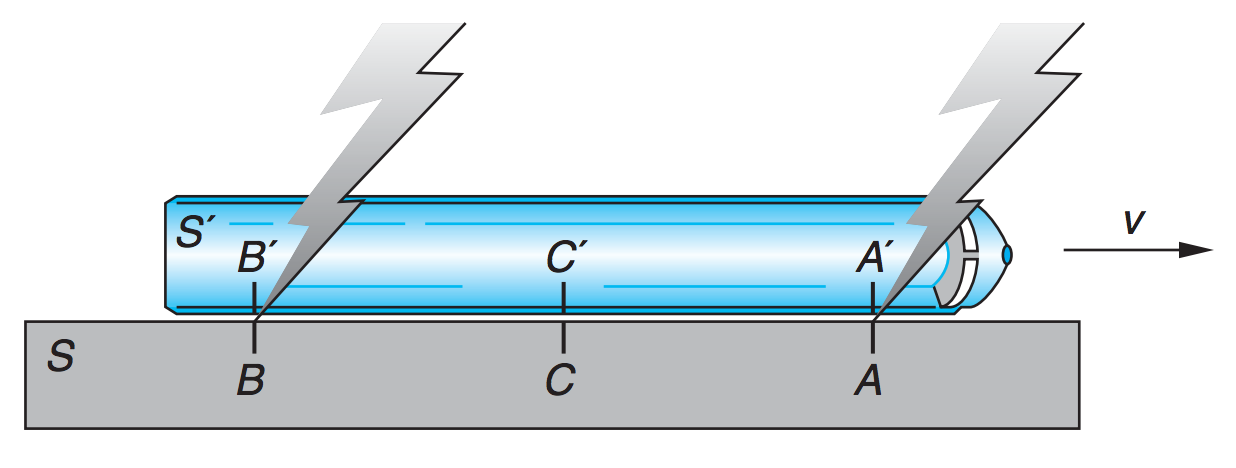
\includegraphics[width=0.7\textwidth]{../images/test2_lightning.png}
	\end{center}
	
	\begin{parts}
		\part A person on the platform says that the distance between \textit{scorched marks on the platform} is \textit{D}. To a person on the train, the distance between \textit{scorch marks on the platform} is:
		\begin{choices}
			\choice Longer than \textit{D}.
			\choice Shorter than \textit{D}.
			\choice Exactly \textit{D}.
			\choice Cannot say, we need more information.
		\end{choices}
		\part A person in the train measures the length of the train to be \textit{L}. To a person on the platform, is the train:
		\begin{choices}
			\choice Longer than \textit{L}.
			\choice Shorter than \textit{L}.
			\choice Exactly \textit{L}.
			\choice Cannot say, we need more information.
		\end{choices}
		\part A person on the platform say that the distance between the \textit{scorch marks on the train} is also \textit{D} (since they see the strikes as happening at the same time). To a person on the train, the distance between \textit{scorch marks on the train} is:
		\begin{choices}
			\choice Longer than \textit{D}.
			\choice Shorter than \textit{D}.
			\choice Exactly \textit{D}.
			\choice Cannot say, we need more information.
		\end{choices}
		\part A person on the platform says the two strikes were simultaneous. What would a person on the train say?
		\begin{choices}
			\choice They would agree, the strikes happened simultaneously.
			\choice They would disagree, and say that the strike at \textit{A'} occurred before the strike at \textit{B'}
			\choice They would disagree, and say that the strike at \textit{B'} occurred before the strike at \textit{A'}
			\choice Cannot say, it is impossible for the person on the train to determine the order the strikes occurred.
		\end{choices}
	\end{parts}
	
	
\clearpage
\question Three electrons have different energies. Using the ideas of wave/particle duality, we can represent the electrons as waves. The following images shows what their wavelength looks like:

\begin{center}
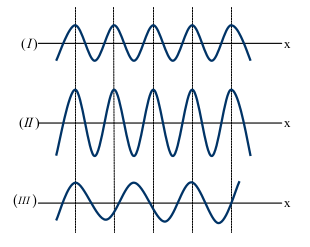
\includegraphics[width=4in]{../images/deBroglie.png}
\end{center}

The following questions will ask about how their energies, $E_I$, $E_{II}$, and $E_{III}$, relate.

\begin{parts}
	\part How do $E_I$ and $E_{II}$ compare?
		\begin{choices}
			\choice $E_{I} = E_{II}$
			\choice $E_{I} > E_{II}$
			\choice $E_{I} < E_{II}$
		\end{choices}
	\part How do $E_I$ and $E_{III}$ compare?
		\begin{choices}
			\choice $E_{I} = E_{III}$
			\choice $E_{I} > E_{III}$
			\choice $E_{I} < E_{III}$
		\end{choices}
	\part How do $E_{II}$ and $E_{III}$ compare?
		\begin{choices}
			\choice $E_{II} = E_{III}$
			\choice $E_{II} > E_{III}$
			\choice $E_{II} < E_{III}$
		\end{choices}
\end{parts}

	\clearpage
	
	\question  You have a jar with 6 red balls and 4 green balls.
\begin{parts}
\part What is the probability of randomly drawing a red ball? What is the probability of randomly drawing a green ball?
\vspace{1.5in}
\part You randomly draw one ball, put it back, and draw a ball again. What is the probability of drawing a red and a green ball, in no particular order?
\vspace{1.5in}
\part You randomly draw one ball then draw another without putting back the first. What is the probability of drawing two red balls?
\vspace{1.5in}
\part You randomly draw one ball then draw another without putting back the first. What is the probability of drawing a red and a green ball, in no particular order?
\vspace{1.5in}
\end{parts}

\clearpage
\question Consider the following experimental setups. Light of a given wavelength is incident on one of two  metal plates sealed inside a vacuum tube. The two plates are connected in circuit to an ammeter, a device that measures electric current. The metal plates have been thoroughly cleaned so that when blue light ($\lambda = 450$~nm) is incident on the lower plate, electrons are ejected.
\begin{parts}
\part There are two lightbulbs, which emit light at 300 nm and 400 nm. These wavelengths are shorter than blue light. Is the energy of the photons emitted by these two lightbulbs:
	\begin{choices}
		\choice The same as the energy contained in blue light (with wavelength 450 nm).
		\choice Greater than the energy contained in a blue light (with wavelength 450 nm).
		\choice Less than the energy contained in a blue light (with wavelength 450 nm).
	\end{choices}
\part In the following two setups, light of 300 nm and 400 nm wavelength (ultraviolet light) is incident on the lower plates. The number of photons landing on the metal plate per second is the same in both setups (they have the same intensity). Compare the number and energy of emitted electrons in the two setups.
\begin{center}
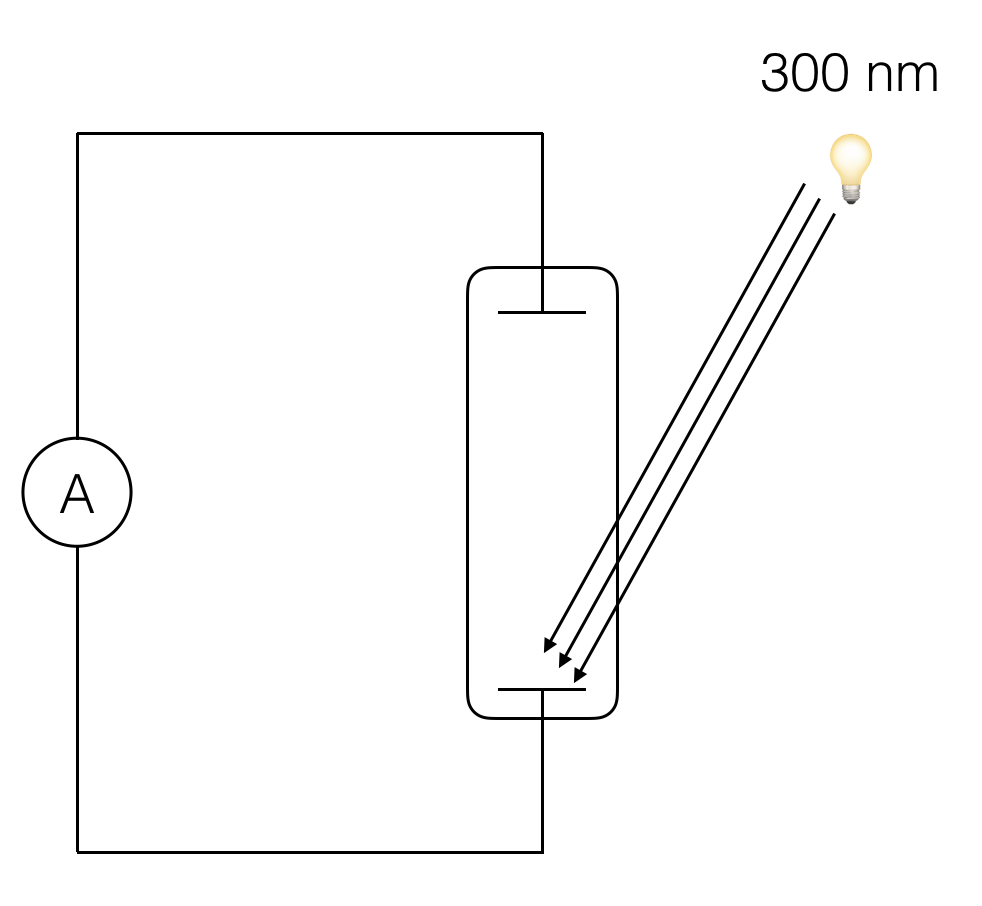
\includegraphics[width=0.45\textwidth]{../images/test2_300nm.png} 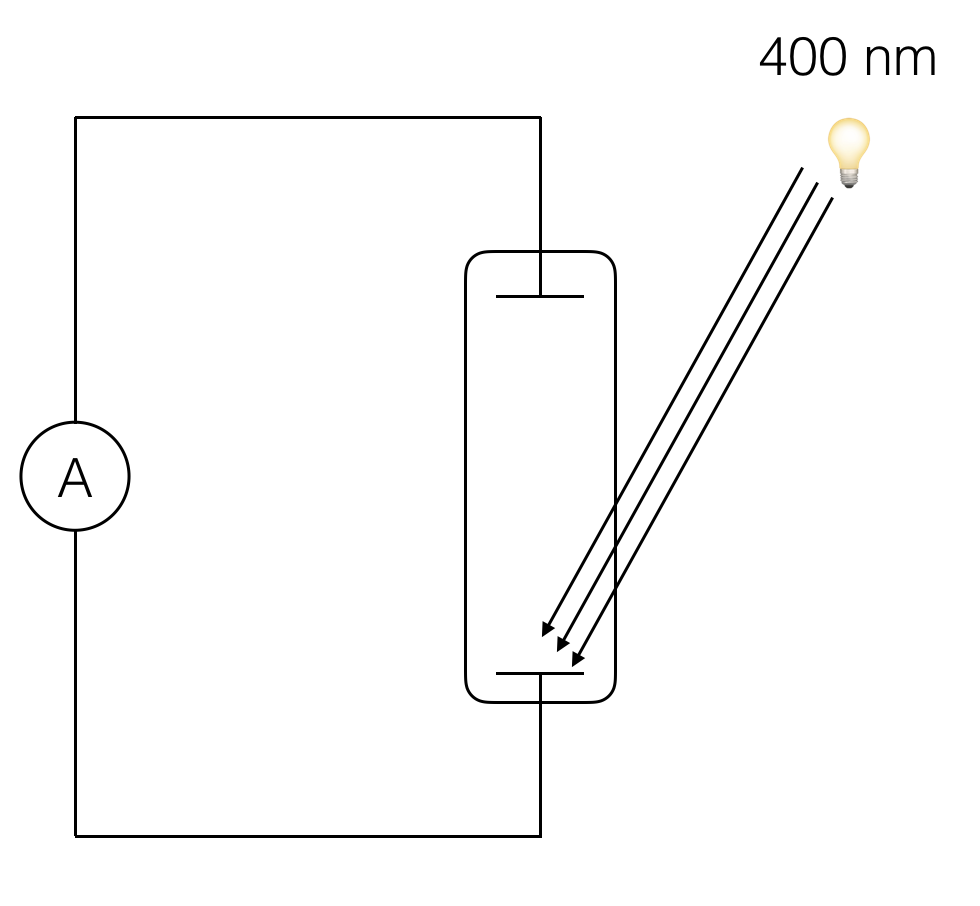
\includegraphics[width=0.45\textwidth]{../images/test2_400nm.png}
\end{center}
	\begin{choices}
		\choice The two setups emit the same number of electrons, however the setup on the left emits electrons with greater energies.
		\choice The two setups emit the same number of electron, however the setup on the right emits electrons with greater energies.
		\choice The two setups emit electrons at the same energies, however the setup on the left emits more.
		\choice The two setups emit electrons at the same energies, however the setup on the right emits more.
		\choice The two setups emit the same number of electrons and at the same energies.
	\end{choices}
\vspace{2in}
\clearpage
\part  In the following two setups, light of 300 nm wavelength (ultraviolet light) is incident on the lower plates. There are three times as many photons landing on the metal plate per second in the setup on the left (the left light has a greater intensity). Compare the number and energy of emitted electrons in the two setups.
\begin{center}
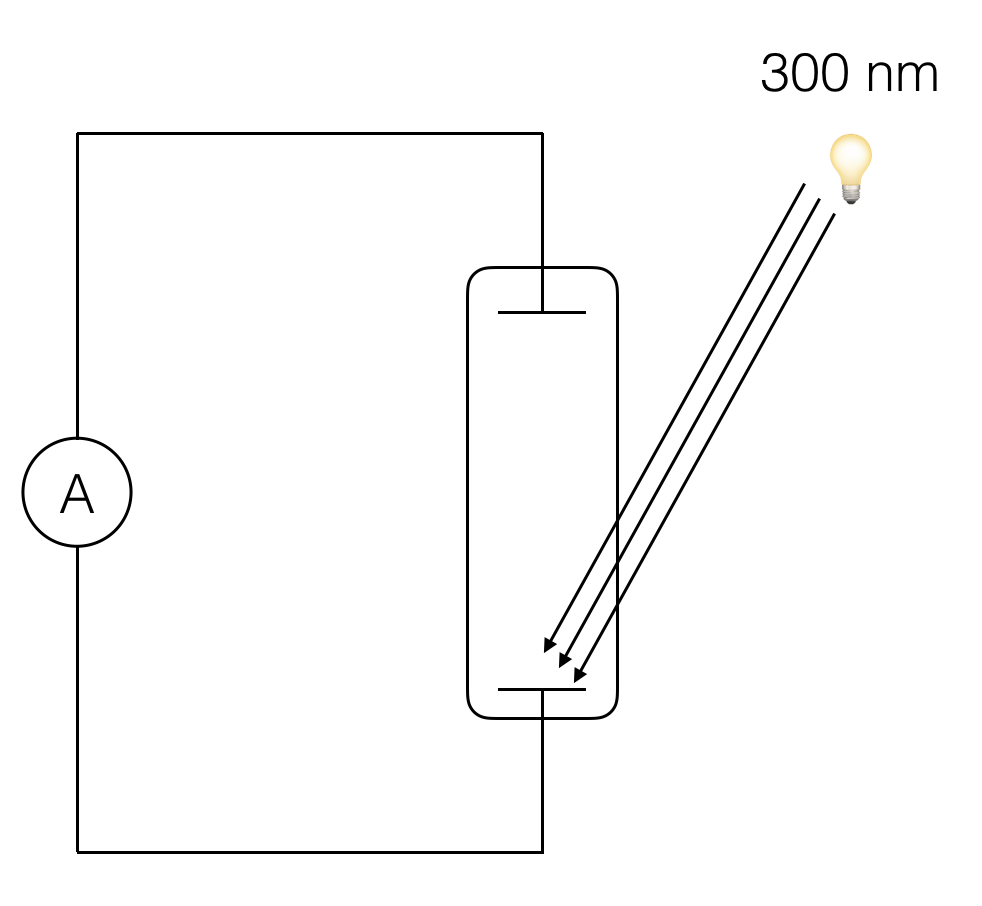
\includegraphics[width=0.45\textwidth]{../images/test2_300nm.png} 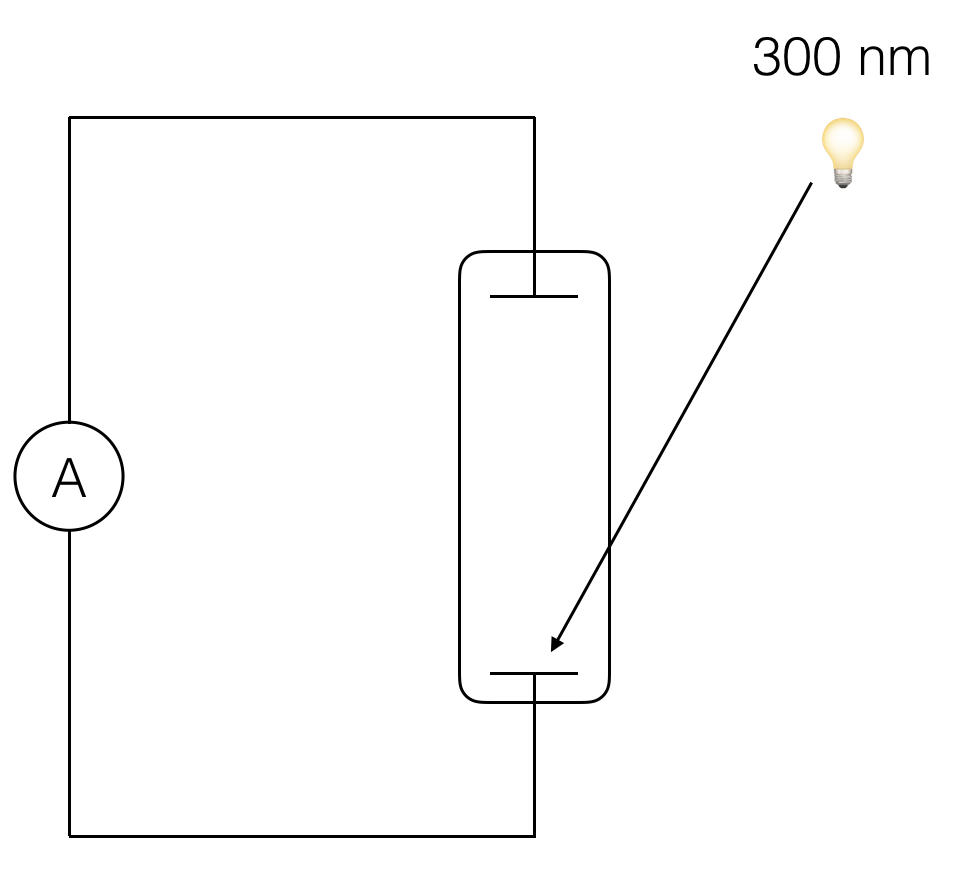
\includegraphics[width=0.45\textwidth]{../images/test2_300nm1.png}
\end{center}
	\begin{choices}
		\choice The two setups emit the same number of electrons, however the setup on the left emits electrons with greater energies.
		\choice The two setups emit the same number of electron, however the setup on the right emits electrons with greater energies.
		\choice The two setups emit electrons at the same energies, however the setup on the left emits more.
		\choice The two setups emit electrons at the same energies, however the setup on the right emits more.
		\choice The two setups emit the same number of electrons and at the same energies.
	\end{choices}

\end{parts}
	
\clearpage
\question A nuclear physicist in a lab wishes to create oxygen. The graph below shows the binding energies for different elements and isotopes:
\noindent\begin{center}
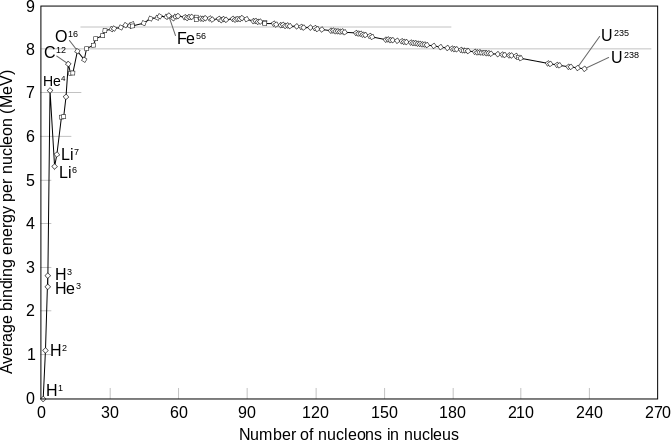
\includegraphics[width=0.9\textwidth]{../images/bindingEnergies.png}
\end{center}
\begin{parts}
	\part She combines $^3He$ to create $^{16}O$. Overall, would this release or require energy?
		\vspace{0.5in}
	\part She breaks apart $^{56}Fe$ to create $^{16}O$. Overall, would this release or require energy?
		\vspace{0.5in}
\end{parts}

\question $^{234}$Pu decays in two different ways:
\begin{enumerate}
	\item Via beta decay, where a neutron become a proton, and in the process emits an electron and an anti-neutrino:
	\begin{eqnarray}
	n \rightarrow p^+ + e^- + \bar{\nu} \nonumber
	\end{eqnarray}
	\item Via alpha decay, where a $^4$He nucleus is emitted.
\end{enumerate}
What are the two different isotopes created as products of these two modes of decay?

From \textit{Light and Matter}, Chapter 26 Question 3.
\vspace{0.5in}

\question Suppose $^{244}$Pu undergoes a perfectly symmetric fission, and in the process emits 2 neutrons. What would be the two daughter nuclei? (Be sure to list the number of protons and neutrons in each).
\vspace{0.5in}

\question The masses of different particles are shown below:

\begin{tabular}{l l }
	proton & $1.67265 \times 10^{-27}$ kg \\
	electron & $0.00091 \times 10^{-27}$ kg \\
	neutron & $1.67495 \times 10^{-27}$ kg\\
	antineutrino & $< 10^{-35}$ kg
\end{tabular}

\begin{parts}
	\part Considering Einstein's equation which relates mass to energy via $E=mc^2$, which particle contains the greatest mass-energy?
		\vspace{0.2in}
	\part Which particle contains the least mass-energy?
		\vspace{0.2in}
	\part By the principle of wave-particle duality, we know that these different particles also have different wavelengths. Below are 4 different waves (not to scale, shown with decreasing wavelength), which represent the wavelengths of these different particles (assuming their velocities are negligible). Label them.
\end{parts}

\begin{center}
	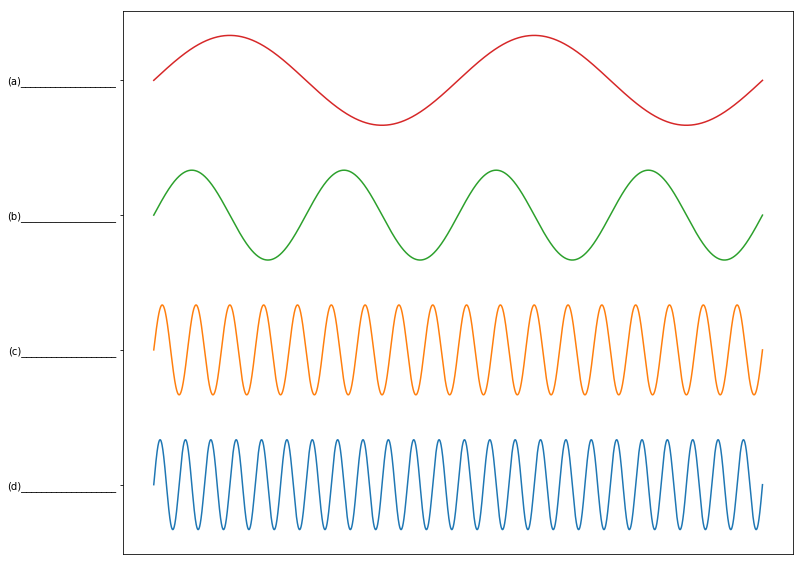
\includegraphics[width=0.9\textwidth]{../images/particleWavelengths.png}
\end{center}	

\clearpage
\question Suppose you have exactly 512 billion radioactive atoms, with a half-life of 10 hours.
	\begin{parts}
		\part How many atoms would you expect to have \textbf{decayed} after 10 hours?
			\vspace{0.5in}
		\part How many atoms would you expect to have \textbf{decayed} after 30 hours?	
			\vspace{0.5in}
		\part Suppose your friend also has exactly 512 billion radioactive atoms, also with a half-life of 10 hours. After 10 hours, how many atoms would they expect to have decayed after 10 hours?
			\vspace{0.5in}
		\part You and your friend count exactly how many atoms had decayed in 10 hours. Would these two numbers be exactly the same? \textbf{Explain.}
			\vspace{0.5in}
	\end{parts}
	
\question The coating on the inside of fluorescent light tubes absorbs ultraviolet light and subsequently emits visible light. An inventor claims he is able to do the reverse process. Is the inventor's claim possible? (Think conservation laws...)
	\vspace{1in}

\question Is the event horizon of a black hole the actual physical surface of the object?

From \textit{College Physics,} Chapter 34 Question 16.
\vspace{1in}

\clearpage
\question Black holes are formed when the \textit{density} of an object becomes so large than space is warped to the point light cannot escape: This means there are very massive black holes (that are many times the mass of our sun) and very small black holes (that can have the mass of an asteroid, compressed to a space small enough). Suppose the moon were to be compressed to the point that it becomes a black hole - how would this effect life on Earth?
\vspace{1in}

\question Suppose we launch a satellite into a black hole. The satellite has on it a blinking light, which we are able to observe from our safe point very far away.

\input{../images/blackHoleProbe.pdf_tex}

\begin{parts}
	\part At which point (a), (b), (c), does the probe experience the strongest gravitational field?
		\vspace{0.2in}
	\part To an observer on Earth, what happens to the time between light flashes (from the blinking light) as the probe goes from (a) to (b) to (c)?
		\vspace{0.2in}
	\part To an observer on Earth, what happens to the wavelength of the light in the light flashes as the probe goes from (a) to (b) to (c)?	
		\vspace{0.2in}
	\part What happens to the time between light flashes when the probe reaches the event horizon?
		\vspace{0.2in}
	\part If someone were on the probe observing people on Earth, what would they see as they approach the event horizon?
		\vspace{0.2in}
\end{parts}

\clearpage
	
\question Light from distant galaxies appears red-shifted, indicating that we are moving apart from each other. Furthermore, the further away an object the more red-shifted it is: Indicating that the universe is expanding. Explain (using the cosmological model of the evolution of the universe) why it only appears that we are at the center of expansion of the universe and why an observer in another galaxy would see the same relative motion in all but the closest galaxies away from her.

From \textit{College Physics}, Chapter 34 Conceptual Question 1.
\vspace{2in}

\question In the beginning of this course, we discussed philosophy of science and the idea that scientific ideas must be falsifiable (meaning, it is possible to design an experiment that would disprove them). 

\begin{parts}
\part As light escapes a gravitational well, it is red-shifted. Galaxies are very massive objects, and have a gravitational field around them (which is why light bends around them). Therefore, if we observe light from a distant galaxy much more dense than our own, we would expect it to be red-shifted (since light would be moving from a large gravitational field to a relatively weaker one here on Earth).

Theoretically, we could use this to explain the redshift in light from distant galaxies, and could therefore disprove the theory that the universe is expanding. Propose an experiment/observation that could disprove this.
\vspace{1in}

\part Propose an experiment/observation that could test between these two theories: (1) Universe is expanding (2) Red-shift in light is due to gravitational fields of distant galaxies.
\end{parts}

\vspace{1in}

\clearpage
\question Imagine you are walking through a forest. You know a tree is in front of you because you can see it (and you know this without needing to test further, say by reaching out and touching it) and so you walk around the tree so as to not walk into it. People who are visually impaired use canes to see, by sweeping the area in front of them. If the cane hits something, they feel the impact on the cane and know to avoid the object - in this way, someone who is blind knows there's a tree in front of them and will walk around it as well.
\begin{parts}
	\part Are these two ways of ``seeing" fundamentally different? Is using a tool to ``see" the world less valid than using our senses?
		\vspace{2in}
	\part We cannot see individual atoms because we are too big, or distant black holes because we are so small. Instead, we rely on tools to probe for us (for atoms, we can look at the Brownian motion of microscopic particles and for black holes we can observe the effect they have on the orbits of stars surrounding them). Do you think this is a valid way to ``see" the universe, or is it too fundamentally different from seeing with our own senses to be comparable?
		\vspace{1in}
\end{parts}

\clearpage
\question You have three fair, six-sided dice. You roll all three of them at once.
\begin{parts}
	\part What is the probability of rolling all 1s? P(1,1,1) = ?
		\vspace{1in}
	\part What is the probability of rolling three of a kind? P(x,x,x) = ?
		\vspace{1in}
	\part What is the probability of rolling a one and two twos? 1, 2, 2
		\vspace{1in}
	\part What is the probability of rolling a one and two of a kind (that aren't ones)? 1,2,2 or 1,3,3 or 1,4,4 or 1,5,5 or 1,6,6
		\vspace{1in}
	\part What is the probability of rolling one, two and a three?
		\vspace{1in}
\end{parts}

\end{questions}

\end{document}
